%-------------------------------------------------------------------------------
% seq64_build
%-------------------------------------------------------------------------------
%
% \file        seq64_build.tex
% \library     Documents
% \author      Chris Ahlstrom
% \date        2015-11-06
% \update      2018-11-08
% \version     $Revision$
% \license     $XPC_GPL_LICENSE$
%
%     Provides the man page section of seq24-user-manual.tex.
%
%-------------------------------------------------------------------------------

\section{Building Sequencer64}
\label{sec:seq64_build}

   The project packaging for \textsl{Sequencer64}
   is aimed at developers.
   But note that we have Debian packages, conventional tarballs,
   and \textsl{Windows} installers in the "Sequencer64
   Packages" project (\cite{sequencer64packages}).
   If one has packages built for other Linux distributions, let us know, and we
   can stick them there for others to use.

   This section presents a how-to on building the various versions of
   \textsl{Sequencer64} from source code.  It's actually pretty easy, with
   these instructions. And please note that there are many ways to build
   \textsl{Sequencer64}, each described in its own section.

\subsection{Linux INSTALL Build}
\label{subsec:seq64_build_install}

   There are many build options.  Some are modifiable via the normal GNU
   \texttt{configure} script method.  Many more are modifiable by
   editing the source code to \textbf{\#define} and \textbf{\#undefine} certain
   macros.  If you don't care about such options, start here.  If you want to
   see what options are available, skip to
   \sectionref{subsubsec:seq64_build_configure}, which has many details one can
   adjust.
   The project includes the conventional GNU \texttt{configure} script, in the
   tarball and in the git-cloned project.  However, the
   the \texttt{bootstrap} script can be used to start from scratch,
   as in the following instructions:

   \begin{enumber}
      \item Preload the dependencies, as listed in
         \sectionref{subsec:seq64_build_dependencies}.
          If some are missing, the
          \texttt{configure} script will tell you,
          or, at worst, a build error will.
      \item Check-out the desired branch, normally "master".
         Make a branch, if desired, to make changes.
         See the file \texttt{git.txt} in the
         \texttt{contrib/notes} project directory.
      \item From the top project directory, run the commands:
\begin{verbatim}
      $ ./bootstrap
      $ ./configure
\end{verbatim}
      \item For debugging without libtool getting in the way, just run
         one of the following commands, which run the
         \texttt{configure} script, adding the
         \texttt{--enable-debug} and
         \texttt{--disable-shared} options to it.
         The bootstrap script is our start-over
         way of setting up GNU autoconf.
\begin{verbatim}
      $ ./bootstrap --enable-debug
      $ ./bootstrap -ed
\end{verbatim}
      \item Run the make command:
\begin{verbatim}
      $ make
\end{verbatim}
      \item To install \textsl{Sequencer64}, become root and run:
\begin{verbatim}
      # make install
\end{verbatim}
   \end{enumber}

   Note that an alternate user-interface (Qt) and alternate MIDI engine
   (portmidi) can be configured and built.
   See \sectionref{subsec:seq64_build_Qt}.
   Also note that one has to build the documentation and Debian packaging
   separately, they are not part of the default build.

%  Please note that there are other things one can do to speed up the build
%  process.
   Noted above is the \texttt{--enable-debug} option.
   The following command bootstraps and then configures
   for release mode, and greatly reduces the amount of compiler output:
 
\begin{verbatim}
   $ ./bootstrap --enable-release
   $ ./bootstrap -er
\end{verbatim}

   This script option runs:

\begin{verbatim}
   $ ./configure --enable-silent-rules
\end{verbatim}

   It results in abbreviated output, which makes it easier to see
   warnings that might pop up.
   This anti-verbosity option can be overridden at "make" time:

\begin{verbatim}
   $ make V=1
\end{verbatim}

   \texttt{V=0} is another way to quiet down the build.
   Note that the build can be sped up by telling \texttt{make}
   to use more cores.
   For example, if one has an 8-core system:

\begin{verbatim}
   $ make -j 8
\end{verbatim}

%  Of course, one can use fewer than the number of cores, if desired.

\subsection{Options for Sequencer64 Features}
\label{subsec:seq64_build_options}

   \textsl{Sequencer64} comes with options for the \texttt{configure} command
   and options represented by definable macros in the source code.

\subsubsection{"configure" Options}
\label{subsubsec:seq64_build_configure}

   The following \texttt{configure} options can be specified on the command
   line:

   \setcounter{ItemCounter}{0}      % Reset the ItemCounter for this list.

   \itempar{\texttt{--enable-rtmidi}}{build!enable rtmidi}
        \index{BUILD\_RTMIDI}
        This option can be bootstrapped directly using
        "\texttt{./bootstrap -er -rm}.
        This is currently the default build.  It creates
%       the default version of \textsl{Sequencer64}, an executable named
        an executable, \texttt{seq64}.
        This version can do JACK input/output
        using the native API... no more need to use \texttt{a2jmidid} to
        bridge from ALSA to JACK.  It provides a JACK client separate
        from the legacy JACK-transport client. \texttt{seq64}
        falls back to using ALSA if JACK is not running.  
        Like ALSA, the JACK support has an auto-connect feature
        that can be disabled using the "manual" ("virtual-port")
        option.

        We term this version "rtmidi" because we originally
        used the RtMidi (\cite{rtmidi}) project as the basis for the native
        JACK support, but it does not quite fit the usage model
        of \textsl{Sequencer64}, so we heavily refactored it.
%       keeping a couple of key features, and keeping the moniker "rtimidi".

   \itempar{\texttt{--enable-qt}}{build!enable qt}
        This sets up a build \textsl{Sequencer64} that uses a Qt
        user-interface.  This version can be build with the RtMidi or PortMidi
        engines.
        Try "\texttt{./bootstrap -er -rm -qt} or
        "\texttt{./bootstrap -er -pm -qt}.

   \itempar{\texttt{--enable-cli}}{build!enable cli}
        \index{BUILD\_RTCLI}
        Bootstrapping directly:
        "\texttt{./bootstrap -er -cli}".
        It sets up a command-line build of \texttt{seq64} that has the
        program name \texttt{seq64cli}.
        This application must be controlled via MIDI controls set up in the
        [midi-control] section of the "rc" file.
        See \sectionref{subsec:seq64_rc_file_midi_control}, for
        information on those controls, which include start, stop,
        pause, play-list navigation, and other commands.
        A single song can be loaded via the last command-line argument.
        A number of songs can be loaded via a play-list.
        See \sectionref{sec:playlist}.
        There is an option to make
        the application fork into the background as a daemon.
%       We're looking in to using OSC as a control mechanism, but the available
%       MIDI control might be sufficient.

   \itempar{\texttt{--enable-alsamidi}}{build!enable alsamidi}
        \index{BUILD\_ALSAMIDI}
        Bootstrapping directly:
        "\texttt{./bootstrap -er -am}".
        This executable is basically the original version of 
        \textsl{Sequencer64}, with the original executable name of
        \texttt{sequencer64}, which we're keeping around as a backup while we
        work the remaining nits out of the "rtmidi" version of the application.

   \itempar{\texttt{--enable-portmidi}}{build!enable portmidi}
        \index{BUILD\_PORTMIDI}
        Bootstrapping directly:
        "\texttt{./bootstrap -er -pm}".
        This option builds the PortMIDI version of the application,
        \texttt{seq64portmidi}.  This version works with
        \textsl{Linux}, but is meant as a way to pre-test the
        port \textsl{seq24} to Windows ("Google" for "seq24 subatomic glue").
%       However, the \textsl{Sequencer64} project
%       deprecates this version.
%       Eventually, we hope to migrate in
%       the Windows and Mac OSX support modules of the RtMidi
%       (\cite{rtmidi}) project.
        This version is used for the \textsl{Windows} and
        \textsl{Mac} ports.

   \itempar{\texttt{--disable-highlight}}{build!disable highlight}
        \index{SEQ64\_HIGHLIGHT\_EMPTY\_SEQS}
        Undefines the \texttt{SEQ64\_HIGHLIGHT\_EMPTY\_SEQS}
        macro, which is otherwise defined by default.  If defined, the
        application highlights empty patterns by coloring them yellow.
%       If not defined, empty sequences/patterns are shown in the normal
%       black-on-white coloring.  In either case, empty patterns will not be
%       played.
        Applies only to the Gtkmm user-interface.

    \itempar{\texttt{--disable-lash}}{build!disable lash}
        \index{SEQ64\_LASH\_SUPPORT}
        Undefines the \texttt{SEQ64\_LASH\_SUPPORT} macro, but it
        is now undefined by default.
        \textsl{Linux} only.
%       Even if this option is left defined,
%       however, \textsl{Sequencer64} will still not use LASH support unless
%       one specifies \texttt{--lash} on the \texttt{sequencer64} command-line or
%       turn on the new \texttt{[lash-session]} option in the "rc"
%       configuration file,
%       \texttt{\textasciitilde/.config/sequencer64/sequencer64.rc}.

    \itempar{\texttt{--disable-jack}}{build!disable jack}
        \index{SEQ64\_JACK\_SUPPORT}
        Undefines the \texttt{SEQ64\_JACK\_SUPPORT} macro, which is
        defined by default.  Even if left defined,
        however, \textsl{Sequencer64} will still not use JACK support unless
        one specifies the various JACK options on the \texttt{sequencer64}
        command-line or turn them on in the "rc" configuration file,
        \texttt{\textasciitilde/.config/sequencer64/sequencer64.rc}.
        \textsl{Linux} only.

    \itempar{\texttt{--disable-jack-session}}{build!disable jack session}
        \index{SEQ64\_JACK\_SESSION}
        Undefines the \texttt{SEQ64\_JACK\_SESSION} macro, which is
        defined if JACK support is defined, and the jack/session.h file is
        found.  Again, this option, if left defined, can be affected by
        command-line options and options in the "rc" configuration file.
        \textsl{Linux} only.

%   \itempar{\texttt{--disable-pause}}{build!disable pause support}
%       \index{SEQ64\_PAUSE\_SUPPORT}
%       This option undefines the \texttt{SEQ64\_PAUSE\_SUPPORT} macro,
%       which is defined by default, and provides support for toggling between
%       a Play button and a Pause button, for actually pausing playback
%       in Live mode, and for a new Pause key, which defaults to a
%       period (".").
%
%   \itempar{\texttt{--disable-chords}}{build!disable chords support}
%       \index{SEQ64\_STAZED\_CHORD\_GENERATOR}
%       This option undefines the \texttt{SEQ64\_STAZED\_CHORD\_GENERATOR}
%       macro.  If this macro is defined,
%       then the application is built with support for a Chord button in the
%       pattern editor, which enables entering whole chords with a single
%       click.  This feature is grabbed from \textsl{Seq32} (\cite{seq32}).
%
%   \itempar{\texttt{--disable-transpose}}{build!disable transpose support}
%       \index{SEQ64\_STAZED\_TRANSPOSE}
%       This option undefines the \texttt{SEQ64\_STAZED\_TRANSPOSE}
%       macro.  If this macro is defined,
%       then the application is built with support for a Transpose button in the
%       pattern editor and the song editor.  The Transpose button in the
%       pattern editor allows a pattern to be exempt from transposition,
%       while the Transpose button in the song editor allows transposing the
%       entire song (except for exempt patterns).
%       This feature is grabbed from \textsl{Seq32} (\cite{seq32}).

    \itempar{\texttt{--disable-multiwid}}{build!disable multi-wid support}
        \index{SEQ64\_MULTI\_MAINWID}
        Undefines the \texttt{SEQ64\_MULTI\_MAINWID} macro.
        If this macro is defined (currently the default), then it is
        possible to show multiple sets in the main window.
        See \sectionref{subsec:seq64_patterns_panel_multiple},
        which describes this mode.  Gtkmm only.

    To summarize, these option macros define/undefine the following build
    macros:

      \begin{itemize}
        \item \texttt{SEQ64\_HIGHLIGHT\_EMPTY\_SEQS}
        \item \texttt{SEQ64\_LASH\_SUPPORT}
        \item \texttt{SEQ64\_JACK\_SUPPORT}
        \item \texttt{SEQ64\_JACK\_SESSION}
%       \item \texttt{SEQ64\_PAUSE\_SUPPORT}
%       \item \texttt{SEQ64\_STAZED\_CHORD\_GENERATOR}
        \item \texttt{SEQ64\_MULTI\_MAINWID}
      \end{itemize}

   A lot of options have become mandatory over the years, and are not discussed
   here.  And there may be more macros not discussed.  For the latest, see the
   \texttt{INSTALL} file in the source-code project.

\subsubsection{Manually-defined Macros in the Code}
\label{subsubsec:seq64_build_macros}

   As we have explored what \textsl{Seq24} does as we improve
   \textsl{Sequencer64}, we've found of things that might change the code
   for the worse in some minds.
   We mark those changes with macros.
   And sometimes we tried a change, but left it
   disabled.  Look at those macros, modify them, and build
   the source code to one's preferences.  If one does not see a macro described
   below, it means we need to catch up with the documentation.

   The following items are not part of the configure script, but can
   be edited manually in the header file
   \texttt{libseq64/include/seq64-features.h}
   to achieve the desired settings:

   \setcounter{ItemCounter}{0}      % Reset the ItemCounter for this list.
   
    \itempar{\texttt{SEQ64\_EDIT\_SEQUENCE\_HIGHLIGHT}}{build!seq highlight}
        Defined in the \texttt{perform} module.
        Provides the option to highlight the currently-editing sequence in the
        main window view and in the song editor.  If the sequence is muted, it
        is highlighted in black text on a cyan background.  If it is unmuted,
        it is highlighted in cyan text on a black background.  The highlighting
        follows whichever pattern editor or event editor has the focus.
        Gtkmm only.

%   \itempar{\texttt{SEQ64\_USE\_NEW\_FONT}}{build!new font}
%       Already defined in the \texttt{font} module.
%       If defined, a new, anti-aliased,
%       bold font is used in the user-interface.  This new font is implemented
%       in new XPM files in \texttt{resources/pixmaps} directory:
%       \texttt{wen*.xpm}.  The font is slightly
%       larger, but changes the user-interface sizes only to an infinitesmal
%       degree.
%       Gtkmm only.
%
%       \textbf{Obsolete:}
%       \index{obsolete:compile-time font}
%       This option is no longer a compile-time option, but a run-time option.
%       It is now the default, but the usage of the old versus new font can be
%       set in the "user" configuration file.
%       Also, if the legacy mode is specified, the old font becomes the
%       default.

    \itempar{\texttt{SEQ64\_USE\_EVENT\_MAP}}{build!event map}
        Already defined in the \texttt{event\_list} module.
        It enables the usage of an
        \texttt{std::multimap}, instead of an \texttt{std::list},
        to store MIDI events.  Because
        the code does a lot of sorting of events, using the
        \texttt{std::multimap} is actually a lot faster (especially under debug
        mode, where it takes
        many seconds for a medium-size MIDI file to load using the
        \texttt{std::list} implementation.
        But the \texttt{std::multimap} can be a limiting factor during playback.
        We use the list implementation and sort the container only after
        getting all the events loaded.

    \itempar{\texttt{SEQ64\_USE\_MIDI\_VECTOR}}{build!midi vector}
        Defined in the \texttt{seq64\_features.h} file.
        It enables the usage of an
        \texttt{std::vector} instead of \texttt{std::list},
        to store MIDI data bytes.
        It provides the preferred alternative to the list for storing and
        counting the bytes of MIDI data.  It stops the reversing of
        certain events due to the peculiarities of \texttt{std::list}.
%       This new implementation uses
%       \texttt{std::vector} and does not use \texttt{pop\_back()} to retrieve
%       the bytes for writing to a file.
%
%   \itempar{\texttt{SEQ64\_FOLLOW\_PROGRESS\_BAR}}{build!follow progress bar}
%       Already defined in the \texttt{app\_limits.h} module.
%       It enables the automatic scrolling (horizontal paging) of the pattern
%       editor and song editor piano rolls, to keep the progress bar in view at
%       all times.  This feature is useful for patterns that are longer than
%       the span of the editor windows.  Such scrolling is a common
%       feature of software MIDI sequencers.
%
%  \textbf{Obsolete}:  Still need to replicate the descriptions that follow
%     in the proper sections.
%
%   \itempar{\texttt{SEQ64\_USE\_GREY\_GRID}}{build!grey/normal grid}
%       \textbf{This item is no longer defined}.
%       Instead, the option is now part of the "rc" configuration file.  This
%       description will be moved to the correct section eventually.
%
%       This configuration item causes the pattern slots/boxes to be colored
%       grey (actually, they will be colored normally as per the current GTK
%       them).  Otherwise, they are colored black.  By default, this value is
%       defined (in the \texttt{mainwid} module).
%
%   \itempar{\texttt{SEQ64\_USE\_WHITE\_GRID}}{build!white grid}
%       \textbf{This item is no longer defined}.
%       Instead, the option is now part of the "user" configuration file.  This
%       description will be moved to the correct section eventually.
%
%       This configuration item causes the pattern slots/boxes to be colored
%       white.  Also definable(in the \texttt{mainwid} module).
%
%   \itempar{\texttt{SEQ64\_USE\_BRACKET\_GRID}}{build!normal grid}
%       \textbf{This item is no longer defined}.
%       Instead, the option is now part of the "user" configuration file.  This
%       description will be moved to the correct section eventually.
%       This configuration box that outlines the pattern slots/boxes is
%       painted over to convert the box to look like a pair of brackets.
%       By default, this value is defined (in the \texttt{mainwid} module).
%
%   \itempar{\texttt{SEQ64\_SEQNUMBER\_ON\_GRID}}{build!grid numbers}
%       \textbf{This item is no longer defined}.
%       Instead, the option is now part of the "rc" configuration file.  This
%       description will be moved to the correct section eventually.
%
%       If the "show sequence numbers" option is on, then each
%       of the blank pattern slots in the main window show the would-be
%       sequence number for that slot.  The background color of the numbers
%       will not match the background color of the grid (which matches the
%       chosen GTK theme).  But, no matter what the GTK background color, they
%       will at least be visible.  There is a little image of this style inside
%       the screenshot shown on the first page of this manual.
%
%       If \texttt{SEQ64\_USE\_WHITE\_GRID}
%       are defined, so that the grid cells are white, then the sequence
%       numbering looks a little nicer, as can be seen in the following
%       figure:
%
% \begin{figure}[H]
%  \centering 
%  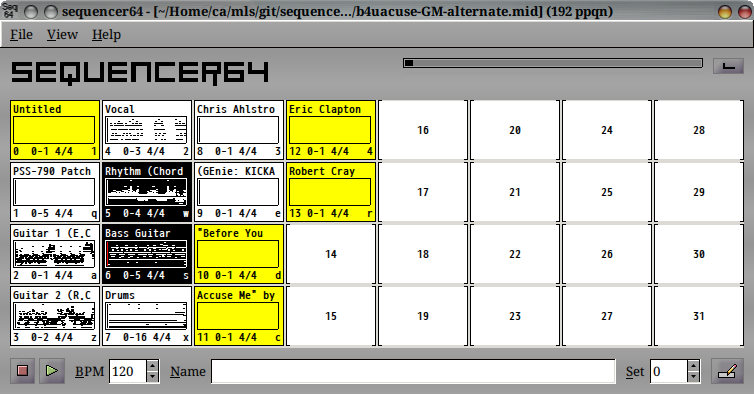
\includegraphics[scale=0.75]{pattern-window-white-box-numbering.png}
%  \caption{Pattern Window Built for White Grid with Numbering}
%  \label{fig:seq64_build_white_box_numbering}
% \end{figure}
%
%       There is a little image of this style inside the screenshot shown on
%       the first page of this manual, as well.
%
%       If neither \texttt{SEQ64\_USE\_GREY\_GRID} nor
%       \texttt{SEQ64\_USE\_WHITE\_GRID} are defined, so that the grid slots
%       are black, then the numbering will be yellow on a black background, and
%       match perfectly.  This style is shown in the following figure:
%
% \begin{figure}[H]
%  \centering 
%  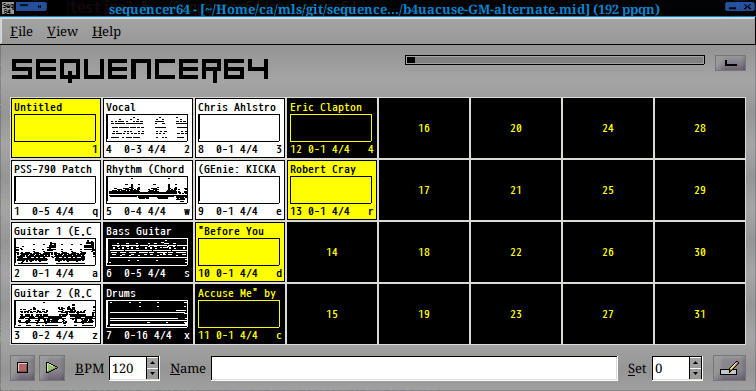
\includegraphics[scale=0.75]{pattern-window-black-box-numbering.png}
%  \caption{Pattern Window Built for Black Grid with Numbering}
%  \label{fig:seq64_build_black_box_numbering}
% \end{figure}
%
%     There is a little image of this style inside the screenshot shown on
%     the first page of this manual, as well.
%
%     Take your pick, modify the code accordingly before building it.
%     Perhaps these can eventually be options for the \texttt{configure}
%     script, or even run-time options!  Let us know!
%
%   \itempar{\texttt{SEQ64\_SOLID\_PIANOROLL\_GRID}}{build!solid piano-roll}
%       Enabling this macro makes the grid lines for the piano rolls
%       more solid, with about the same perception of lightness.
%       It also calls in some other tweaks, such as the positioning of
%       markers.  We currently like this look a little better, and so it is
%       the default.  See the \texttt{app\_limits.h}
%       header file for the definition of this variable.
%
%       Here is the pattern editor (sequence editor) with this alternate look.
%
% \begin{figure}[H]
%  \centering 
%  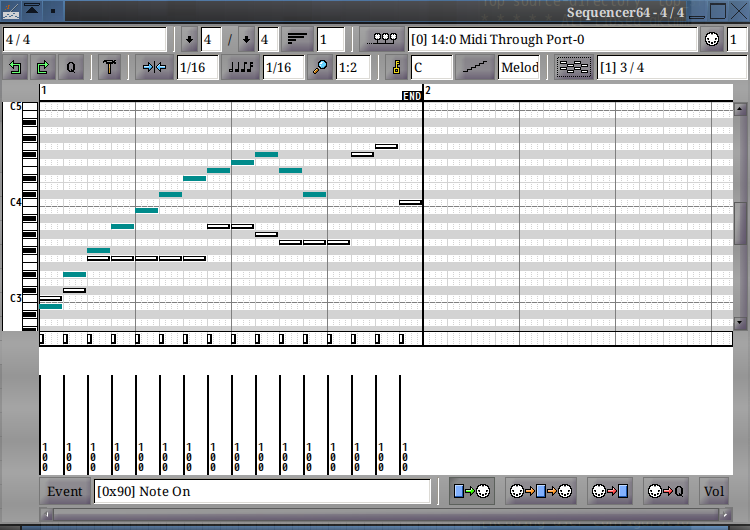
\includegraphics[scale=0.75]{pattern/pattern-editor-alternate-look.png}
%  \caption{Sequence Pattern Editor Alternate Look}
%  \label{fig:seq64_pattern_editor_alternate_look}
% \end{figure}
%
%       Note the smmoothness of the grid lines, the extra emphasis of the C
%       notes at each octave, the emphasis of the note-drawing snap lines that
%       mark the default length of a click-to-add note, the emphasis of the
%       beat and bars, and, finally, the new location of the
%       \textbf{END} marker.  Also note the dark-cyan background pattern,
%       discussed elsewhere in this document.
%
%       Here is the grid-styling for an 8/4 time signature in the song editor:
%
% \begin{figure}[H]
%  \centering 
%  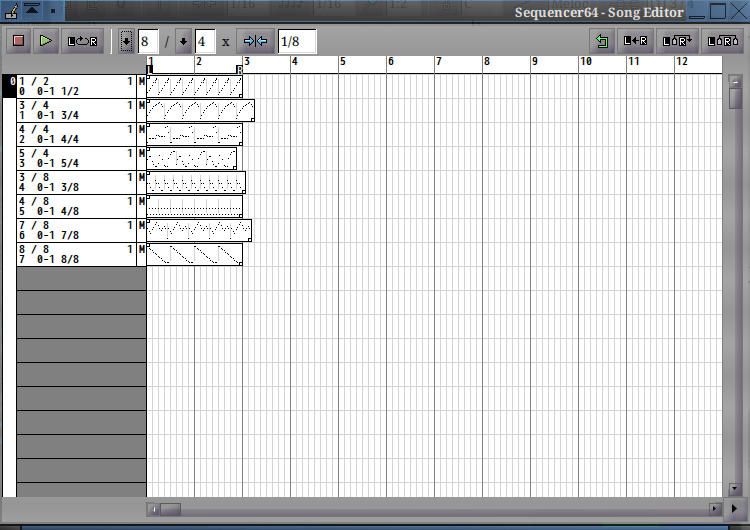
\includegraphics[scale=0.75]{song-editor/song-editor-alternate-look.png}
%  \caption{Song Editor Alternate Look}
%  \label{fig:seq64_song_editor_alternate_look}
% \end{figure}
%
%     Also note the sequence numbers shown in the bottom left of each pattern
%     name box. This is a new feature, and, as noted elsewhere, is a new
%     option in the \textsl{File / Options / Keyboard} tab and in
%     the "rc" configuration file.
%
%   \itempar{\texttt{SEQ64\_USE\_VI\_SEQROLL\_MODE}}{build!vi seqroll}
%       Definable in the seqroll module, this macro allows the vi hjkl keys to
%       be used as arrow keys for moving notes.  Not yet tested.  We will not
%       make this a default, because it could drive non-vi users nuts.

   \itempar{\texttt{SEQ64\_USE\_DEBUG\_OUTPUT}}{build!debug output}
      Enable this macro in the
      \texttt{globals.h} header file, to see extra console
      output if the application is compiled for debugging.  This macro can be
      activated only if \texttt{PLATFORM\_DEBUG} is defined, which is taken
      care of by the build process.  If set, this macro turns on extra
      console output for some modules.

%       \begin{itemize}
%          \item \texttt{globals}
%          \item \texttt{jack\_assistant}
%          \item \texttt{optionsfile}
%          \item \texttt{user\_settings}
%       \end{itemize}

      \index{PLATFORM\_DEBUG}
      Again, note the macro \texttt{PLATFORM\_DEBUG},
      defined in \texttt{platform\_macros.h} if the application is
      built in debug mode.

\subsection{Sequencer64 Build Dependencies}
\label{subsec:seq64_build_dependencies}

   With luck, the following dependencies will bring in their own
   dependencies when installed.  Build requirements:

     \begin{itemize}
        \item libgtkmm-2.4-dev (dev is the header-file package)
        \item libsigc++-2.0-dev
        \item libjack-jackd2-dev
        \item liblash-compat-dev (optional)
     \end{itemize}

   Runtime requirements:

     \begin{itemize}
        \item libatk-adaptor (and its dependencies)
        \item libgail-common (and its dependencies)
        \item valgrind (optional, very useful for debugging)
        \item gdb (optional, very useful for debugging)
        \item gprof and gcov (optional, very useful for debugging)
     \end{itemize}

   Build tools requirements:

     \begin{itemize}
        \item automake and autoconf
        \item autoconf-archive
        \item g++
        \item make
        \item libtool
     \end{itemize}

   Documentation requirements (very optional):

     \begin{itemize}
        \item doxygen and doxygen-latex
        \item graphviz
        \item texlive
     \end{itemize}
      
   Debian packaging (optional):

     \begin{itemize}
        \item debhelper
        \item fakeroot
     \end{itemize}

\subsection{Linux Qt Builds}
\label{subsec:seq64_build_Qt}

   The \textsl{Linux} version of \textsl{Sequencer64} can be built with the Qt
   user-interface, using either the PortMIDI or RtMIDI (preferred) MIDI
   engines.
 
\begin{verbatim}
   $ ./bootstrap --enable-release -rm -qt
   $ ./bootstrap -er -rm -qt
   $ ./bootstrap --enable-release -pm -qt
   $ ./bootstrap -er -pm -qt
\end{verbatim}

   Eventually, the Qt and RtMIDI combination will be the official version
   of \textsl{Sequencer64} for \textsl{Linux}.
   Our PortMIDI engine, while modestly improved over legacy PortMIDI, is not
   quite as complete as our RtMIDI-derived implementation.

\subsection{Linux Qmake Build}
\label{subsec:seq64_build_qmake}

   We wanted to build \textsl{Sequencer64 for Windows} using GNU tools and the
   MSYS platform on either \textsl{Linux} (cross-compiling) or
   \textsl{Windows}.  But it proved more foolproof to create the
   \texttt{*.pro} files necessary for \textsl{qmake} and be able to build
   on \textsl{Windows} and \textsl{Mac OSX}.
   \index{Qt Creator}
   \index{qtcreator}
   This setup and build can be done through \textsl{Qt Creator}.
   The command-line setup is straightforward.
   From the \textsl{Sequencer64} directory, run the following
   commands, using either the build directory specified by \textsl{Qt Creator},
   or making your own "shadow build" directory.

   \begin{verbatim}
        $ mkdir debug-build
        $ cd debug-build
        $ qmake -makefile -recursive "CONFIG += debug" ../sequencer64/qpseq64.pro
        $ make
   \end{verbatim}

    One can also use "CONFIG += release", or just leave that off entirely.

    The \texttt{qpseq64.pro} file can also be loaded in the
    nice IDE, \textsl{Qt Creator}, and be configured, built, and debugged
    there.  And one can tweak the GUI elements in that IDE.

\subsection{Windows Qmake Build}
\label{subsec:seq64_build_qmake_windows}

   The easiest option for a build on \textsl{Windows} is to install 
   \textsl{Qt Creator} in its open-source edition.
   The executable name is
   \texttt{qt-unified-windows-x86-3.0.5-online.exe} or somesuch.
   Rather than navigate through the corporate pages, just go to
   \url{https://download.qt.io/archive/online_installers/3.0/} and
   pick the latest version.
   
   When installing, be sure to select at least the the 32-bit Mingw tools,
   including \texttt{mingw32-make.exe}, and
   \texttt{qmake.exe}.  The \textsl{Windows}
   \textbf{PATH} must be modified to
   include the path to both executables, and the excutables
   \texttt{moc.exe}, \texttt{uic.exe}, \texttt{rcc.exe}, and
   \texttt{windeployqt.exe}.
   If the installation directory for \textsl{Qt Creator} is
   \texttt{ProgramFiles} (e.g. \texttt{C:/Program Files}), then add
   these directories to the user or system PATH:

   \begin{verbatim}
      %ProgramFiles%\Qt\5.11.1\mingw53_32\bin
      %ProgramFiles%\Qt\Tools\mingw530_32\bin
   \end{verbatim}

   Obviously, the version number might differ from "5.11.1".
   There is a build script in the \texttt{nsis} directory that
   automates the process of making the executable:
   \texttt{build\_release\_package.bat}.
   It also shows the steps needed to do a release build and create a
   \textsl{7-Zip} package, which include editing some macro variables with
   naming or version information.  If one wants to do it manually,
   follow these steps.  (We denote the DOS backslash path separator
   by "/", for our convenience.)

   \begin{enumerate}
      \item Using
         "git clone https://github.com/ahlstromcj/sequencer64.git"
         or the unpacking of a source-code tarball,
         create the \texttt{sequencer64} directory with all
         of the project files.
      \item Change to the directory above this directory.
      \item Create an empty "shadow" directory, e.g. \texttt{seq64-release}.
      \item Change to this "shadow" directory.  In that directory, run the
         following command:
         \texttt{qmake -makefile -recursive "CONFIG += release"
            ../sequencer64/qpseq64.pro}.
      \item Next, run the following command and wait for the build to
         complete:
         \texttt{mingw32-make > make.log 2>\&1}.
      \item Open \texttt{make.log} and make sure there are no errors.
         Note that the output directory is inside the "shadow" directory and
         is called \texttt{Seq64qt5/release}.
      \item Run the following command to copy necessary \textsl{Qt} DLLs to
         this directory: \linebreak
         \texttt{windeployqt Seq64qt5/release}.
      \item Create the \texttt{data} directory in
         \texttt{windeployqt Seq64qt5/release} and copy some data files:
         \begin{enumerate}
            \item \texttt{mkdir Seq64qt5/release/data}
            \item \texttt{copy ../sequencer64/data/*.rc Seq64qt5/release/data}
            \item \texttt{copy ../sequencer64/data/*.usr Seq64qt5/release/data}
            \item \texttt{copy ../sequencer64/data/*.midi Seq64qt5/release/data}
            \item \texttt{copy ../sequencer64/data/*.pdf Seq64qt5/release/data}
            \item \texttt{copy ../sequencer64/data/*.txt Seq64qt5/release/data}
            \item \texttt{copy ../sequencer64/data/*.playlist Seq64qt5/release/data}
         \end{enumerate}
      \item Change to the \texttt{Seq64qt5} directory and run:
         \texttt{7z a -r qpseq64-release-package-0.96.1.7z \linebreak release/*}
   \end{enumerate}

   \index{portable package}
   At this point, the \texttt{7z} file is useful as a "portable" package
   for the application.  It can also be used to build the installer, as
   shown in the next section.

   By the way, we have not tried using the Microsoft C++ compiler yet.
   If you try it and get the code to work, let us know!

\subsubsection{Windows Installer}
\label{subsec:seq64_build_installer_windows}

   Here, we unpack the \texttt{7z} release package and then use
   \textsl{NSIS} to build the installer.
   These steps equire \textsl{7-Zip}
   to be installed and accessible from the DOS
   command-line, as \texttt{7z.exe}.
   Requires \textsl{NSIS 3} to be installed, unless one wants to use
   NSIS on Linux to build the installer (our preferred method).
   We build the installer in \textsl{Linux} using the
   \textsl{nsis} package.  These instructions can be adopted to using the
   \textsl{Windows} GUI interface for \textsl{NSIS}.

   \begin{enumerate}
      \item Copy the file
         \texttt{7z a -r qpseq64-release-package-0.96.1.7z} to
         the top-level project directory, \texttt{sequencer64}.
      \item Run
         \texttt{7z x qpseq64-release-package-0.96.1.7z} to extract
         the contents to the \texttt{release} directory.
      \item Run the following commands:
         \begin{enumerate}
            \item \texttt{pushd nsis}
            \item \texttt{makensis Seq64Setup.nsi}
            \item \texttt{popd}
         \end{enumerate}
      \item Verify that the installer works.  It's name is like:
         \texttt{sequencer64\_setup\_0.96.1.exe}
   \end{enumerate}

   The \textsl{bash} script \texttt{packages} does all this, plus
   creates the source-tarball and some other actions for the developers.

%-------------------------------------------------------------------------------
% vim: ts=3 sw=3 et ft=tex
%-------------------------------------------------------------------------------
